\documentclass[british,titlepage]{ntnuthesis}

\usepackage{listings-solidity} % copy listings-solidity.sty to your project

\usepackage{xcolor}
\definecolor{verylightgray}{rgb}{.97,.97,.97}

\lstset{ % define general preferences
	backgroundcolor=\color{verylightgray},
	extendedchars=true,
    showstringspaces=false,
    showspaces=false,
    tabsize=4,
}

\title{EduWallet: A Blockchain-Enabled Digital Wallet for Managing University Course Credits}
\shorttitle{EduWallet}
\author{Diego Da Giau}
\date{2025-05-01}

\addbibresource{thesis.bib}


% From https://www.overleaf.com/learn/latex/Glossaries

\makeglossaries % Prepare for adding glossary entries

\newglossaryentry{application programming interface}{
        name=Application Programming Interface,
        plural=application programming interfaces,
        description={A set of rules and protocols that allow different software applications to communicate with each other, enabling them to exchange information or functionalities}
}

\newglossaryentry{mempool}{
    name=mempool,
    plural=mempools,
    description={Short for memory pool. In general computing, it refers to a temporary memory area used to manage pending operations. In the context of blockchain and account abstraction, a mempool is a temporary storage area to hold UserOerations that have been broadcast to the network but are not yet included in a block}
}

\newglossaryentry{salt}{
    name=salt,
    plural=salts,
    description={A salt is a random sequence of data used in cryptography. It is added to a password before hashing, with the purpose of making the resulting hash unique, even if two users have the same password}
}

\newglossaryentry{keccak256}{
    name=Keccak-256,
    description={A cryptographic hash function that belongs to the Keccak family. It produces a fixed 256-byte hash},
}

\newglossaryentry{nonce}{
    name=nonce,
    plural=nonces,
    description={A nonce is a number that can be used only once in a cryptographic communication. In \acrlong{eth}, the nonce represents the number of transactions sent by a specific address and is used to ensure the uniqueness and validity of each transaction},
}

\newglossaryentry{hash}{
    name=hash,
    plural=hashes,
    description={In computer science, a hash function is an algorithm that takes an input of arbitrary length and produces a fixed-size output, commonly referred to as a hash or digest},
}

\newglossaryentry{double-spending}{
    name=double-spending,
    description={The double-spending problem refers to the malicious act of spending the same digital currency multiple times. In digital systems without adequate safeguards, this vulnerability could allow users to duplicate funds and undermine the integrity of the monetary system},
}

\newglossaryentry{p2p}{
    name=peer-to-peer,
    description={A peer-to-peer network is a distributed system architecture in which all participating nodes, called peers, have equal authority and responsibility},
}

% --------------------
% ----- Acronyms -----
% --------------------

\newacronym{ew}{EW}{EduWallet}
\newacronym{lms}{LMS}{Learning Management System}
\newacronym{api}{API}{\gls{application programming interface}}
\newacronym{sw}{SW}{Smart Wallet}
\newacronym{sdk}{SDK}{Software Development Kit}
\newacronym{cli}{CLI}{Command Line Interface}
\newacronym{ipfs}{IPFS}{InterPlanetary File System}
\newacronym{cid}{CID}{Content Identifier}
\newacronym{url}{URL}{Uniform Resource Locator}
\newacronym{ui}{UI}{User Interface}
\newacronym{gui}{GUI}{Graphical User Interface}
\newacronym{ux}{UX}{User Experience}
\newacronym{ects}{ECTS}{European Credit Transfer and Accumulation System}
\newacronym{eth}{ETH}{Ethereum}
\newacronym{evm}{EVM}{Ethereum Virtual Machine}
\newacronym{eoa}{EOA}{Externally Owned Account}
\newacronym{sca}{SCA}{Smart Contract Account}
\newacronym{it}{IT}{Information Technology}
\newacronym{abi}{ABI}{Application Binary Interface}
\newacronym{aws}{AWS}{Amazon Web Services}
\newacronym{pdf}{PDF}{Portable Document Format}
\newacronym{fr}{FR}{Functional Requirement}
\newacronym{nfr}{NFR}{Non-Functional Requirement}
\newacronym{www}{WWW}{World-Wide Web}
\newacronym{btc}{BTC}{Bitcoin}
\newacronym{dapp}{dApp}{decentralized application}
\newacronym{mit}{MIT}{Massachusetts Institute of Technology}
\newacronym{dcc}{DCC}{Digital Credential Consortium} % add glossary and acronym lists before document

\begin{document}

% \chapter*{Abstract}

% \chapter*{Sammendrag}
Mens verden raskt går fra tradisjonelle Web 2.0-systemer, dominert av store selskaper som tjener penger på sentraliserte data, til Web3-løsninger basert på blockchain-teknologiens desentraliserte natur, er akademia fortsatt i stor grad avhengig av sentraliserte databaser og statiske dokumenter, enten digitale eller på papir. Denne utdaterte tilnærmingen hindrer deling av akademiske opplysninger mellom institusjoner, som ofte krever produksjon, validering og verifisering av dokumenter, samt enighet om felles formater.

Dette arbeidet foreslår en løsning for å modernisere forvaltningen av akademiske opptegnelser. Ved å utnytte blockchain og Ethereum smart contracts legger vi grunnlaget for et system basert på sikre og manipulasjonssikre teknologier. Gjennom bruk av kontoabstraksjon er vi i stand til å utvikle en brukervennlig løsning som muliggjør gasless interaksjoner for brukerne. EduWallet er avhengig av et Software Development Kit (SDK) som gjør det mulig for universiteter å samhandle med on-chain-funksjonaliteter, og en nettleserutvidelse som gjør det mulig for studenter å administrere sine data. En viktig funksjon i den foreslåtte løsningen er full dataeierskap, som i sin helhet gis til studentene, som kontrollerer tilgangen til sine akademiske opplysninger. I tillegg brukes et desentralisert lagringssystem til å lagre studentenes sertifikater, noe som minimerer behovet for lagring av data på kjeden.

EduWallet har som mål å tilby et omfattende miljø innenfor akademiske institusjoner, slik at universitetene kan effektivisere byråkratiske prosesser og tilpasse seg de nyeste Web3-standardene. Den foreslåtte løsningen fungerer også som et praktisk eksempel på hvordan man effektivt kan integrere on-chain- og off-chain-komponenter i et sammenhengende system.

\tableofcontents
\listoffigures
\listoftables
\lstlistoflistings

\printglossary[type=\acronymtype] % Print acronyms
\printglossary                    % Print glossary

% \chapter{Introduction}
\label{chap:introduction}
We are currently living in a globalized world, where distance is increasingly irrelevant. People move freely across borders, and thanks to digital technologies, everyone is interconnected and can access services regardless of location. Schools and universities are deeply affected by this globalization, and their internal operations are rapidly evolving. Today, many students receive education from a variety of sources, often through online courses offered by institutions in different countries. 
A further driver of this change is the rise of academic mobility programs, such as the Erasmus program, an initiative by the European Union designed to promote student and faculty exchanges and foster intercultural experiences.

However, these opportunities introduce challenges in managing and sharing students' academic records. Typically, each university maintains its own format and system for storing academic data, which creates friction when this information needs to be exchanged. When a student transfers to another institution or participates in an exchange program, they must present verified academic documentation, including diplomas and course transcripts. Currently, students are required to request certified digital or paper documents from their home institution, which must be signed and validated by the university. They then submit these to the receiving institution, which must verify the authenticity of both the data and the signatures. This multi-step process is burdensome for both students and universities, involving significant administrative overhead and document handling.

Given our experience with the Erasmus exchange program, and the tedious process of requesting documentation, waiting for it, and resolving discrepancies between universities regarding content and validation, we decided to develop this project. The aim of this thesis is to provide both students and universities with a unified system for storing and sharing academic records. \gls{ew} leverages blockchain technology, utilizing its tamper-proof and verifiable nature to allow universities to securely issue academic records and certificates, while enabling students to access them through ownership of an academic wallet in which the records are stored. User interaction is a central focus of this work, as the solution is intended for students of all backgrounds, without requiring specific computer science skills. Therefore, the system is designed to abstract the complexity of its blockchain-based core.

The remainder of this document is structured as follows: the next chapter, \cref{chap:background}, provides the necessary background information on blockchain and the technologies used within \gls{ew}. \cref{chap:relatedWork} presents the related work. Based on the context established in the previous chapters, \cref{chap:problemStatement} explains the problem addressed in this thesis and introduces the use cases that guided the system design. \cref{chap:requirements} outlines the requirements derived from these use cases.
The design of the proposed solution is presented in \cref{chap:systemArchitecture}, which gives an overview of the components that make up \gls{ew}, and is further detailed in \cref{chap:onchainDesign} and \cref{chap:offchainDesign}, which describe the on-chain and off-chain elements, respectively. The tools and code used for the development of the system are discussed in \cref{chap:implementation}.
A discussion on the solution and the outcomes of this work is provided in \cref{chap:validation}. Finally, \cref{chap:conclusion}  concludes the thesis by summarizing its main contributions and \cref{chap:futureWork} presents directions for future research.
% \chapter{Background Material}
\label{chap:background}
The aim of this chapter is to provide the reader with the fundamentals concepts necessary to understand discussed in this work. All the background knowledge presented here is related to emerging decentralized technologies, which are leveraged to modernize the university system in line with Web3 paradigm.

The chapter begins by tracing the evolution of the internet and websites, from the earliest technologies to today's decentralized web. It then delves into blockchain technologies, with a particular focus on one of the most prominent platforms, \acrlong{eth}. The final section explores decentralized storage solutions, which serve as a bridge between fully on-chain systems and traditional web-based services.

%%%%%%%%%%%%%%%%%%%%%%%%%%%%%%%%%%%%%%%%%%%%%%%%%%%%%%%%%%%%%%%%%%
% FROM WEB 1.0 TO WEB3
%%%%%%%%%%%%%%%%%%%%%%%%%%%%%%%%%%%%%%%%%%%%%%%%%%%%%%%%%%%%%%%%%%
\section{From Web 1.0 to Web3}
The \acrfull{www} \cite{berners1992world} was launched in 1991 with the publication of the first website\footnote{\url{https://info.cern.ch/}} by the English computer scientist Tim Berners-Lee. The goal behind the \acrshort{www} was to create a digital archive of collective human knowledge, accessible to anyone, everywhere. The first iteration of the web is known as Web 1.0, that was composed primarily of static web pages \cite{choudhury2014world}, where users' main activities were limited to reading content created by technically skilled individuals or interacting via emails and chat rooms \cite{murray2023promise}. A major limitation of this model was the stateless nature of protocols like HTTP, which prevented websites from storing or recall user data. As a result, web pages were static and offered limited interactivity, making them unattractive for commercial purpose since monetization was difficult.

Web 2.0 emerged to address these issues by introducing dynamic websites to the \acrshort{www}. In the early 1990s, Lou Montulli, a developer at Netscape, introduced browser cookies \cite{kristol1997rfc2109}, small data files stored by web pages to retain user information. This innovation enabled websites to become dynamic, offering personalized experiences based on user behaviour and preferences. It also paved the way for monetization, as companies could now track and analyse their data. Web 2.0 gave rise to modern tech giants such as Google and Microsoft, whose business models heavily rely on collecting and leveraging user data. However, this shift led to a new issue: user data became the property of centralized platforms, which could exploit or sell it without users' consent.

Web3 aims to reverse this trend by decentralising data ownership and returning control to the users \cite{sheridan2022web3}\cite{ray2023web3}. In the Web3 paradigm, individuals can own their data and choose how it is shared or monetized. The core technology enabling this transformation is the blockchain, a distributed ledger that facilitates interactions with digital services without relying on centralized structures.

%%%%%%%%%%%%%%%%%%%%%%%%%%%%%%%%%%%%%%%%%%%%%%%%%%%%%%%%%%%%%%%%%%
% BLOCKCHAIN
%%%%%%%%%%%%%%%%%%%%%%%%%%%%%%%%%%%%%%%%%%%%%%%%%%%%%%%%%%%%%%%%%%
\section{Blockchain}
A blockchain \cite{nofer2017blockchain} is a linked structure composed of data packages called blocks (hence the name blockchain). Each block contains multiple operations, known as \textit{transactions}, along with metadata such as the cryptographic \gls{hash} of the previous block. This structure links each block to its predecessor, forming the chain depicted in \cref{fig:blockchainStructure}, ensuring the integrity of the entire ledger. Since each block includes the \gls{hash} of the previous one, tampering with a block would require altering all the subsequent blocks in the chain, making such modifications computationally infeasible. 

\begin{figure}
  \centering
  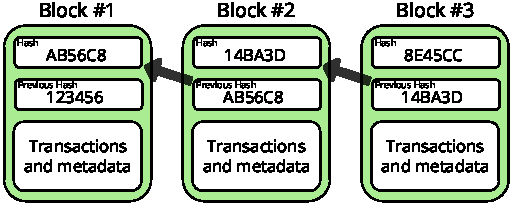
\includegraphics[width=0.7\textwidth]{figures/blockchain.pdf}
  \caption[Blockchain structure]{Blockchain structure showing the chain of blocks.}
  \label{fig:blockchainStructure}
\end{figure}

Blockchains are typically maintained by a \gls{p2p} network, where each participant, referred to as \textit{node}, stores a copy of the blockchain. This decentralized replication ensures data availability, fault tolerance, and security. Nodes follow a consensus protocol, which defines the rules by which transactions are validated and blocks are added to the chain. 

The first blockchain was introduced in 2008 by Satoshi Nakamoto, the pseudonymous creator (or group of creators) of Bitcoin \cite{nakamoto2008bitcoin}. It continues to function as the public ledger for all \acrlong{btc} transactions, effectively solving the \gls{double-spending} problem without the need for a centralized authority. Another widely known blockchain is \acrfull{eth}, which operates alongside its native cryptocurrency, Ether.

%%%%%%%%%%%%%%%%%%%%%%%%%%%%%%%%%%%%%%%%%%%%%%%%%%%%%%%%%%%%%%%%%%
% ETHEREUM
%%%%%%%%%%%%%%%%%%%%%%%%%%%%%%%%%%%%%%%%%%%%%%%%%%%%%%%%%%%%%%%%%%
\section{Ethereum}
\acrlong{eth}\footnote{\url{https://ethereum.org}} was launched in 2015 based on an idea of Vitalik Buterin \cite{buterin2014next}\cite{wood2014ethereum}. Buterin's vision was to enable the deployment of \acrfull{dapp}, programs that run autonomously on a blockchain without relying on external, centralized infrastructure. To realize this vision, he and his collaborators created the \acrfull{evm}, a decentralized virtual machine that executes transactions. In contrast to \acrlong{btc}'s limited instruction set, the \acrshort{evm} supports a broad range of operations, including loops and conditional statements. This flexibility makes it possible to develop \textit{smart contracts}, which are programs containing both code and data that execute on the \acrlong{eth} blockchain.

When users perform on-chain operations, such as sending cryptocurrency or invoking a smart contract function, they consume computational resources. To compensate nodes for providing these resources and to prevent abuse (for example, infinite loops), Ethereum measures resource usage in units called \textit{gas}. Each individual operation requires a specific amount of gas, and the total \textit{gas fee} for a transaction is calculated by multiplying the gas used by the current \textit{gas price}. Because gas is paid in Ether, the cost of executing an operation varies with the market value of Ether.

Users hold Ethers and pay transaction fees via \acrfull{eoa}, which can initiate transactions and serve as the interface between users and the blockchain. An \acrshort{eoa} is derived from a private key, which is also required to cryptographically sign transactions. The other account type in Ethereum is the \textit{contract account}, which corresponds to a deployed smart contract. Contract accounts can hold cryptocurrency but cannot initiate transactions on their own; they can only send transactions in response to receiving one. Both contract accounts and \acrshort{eoa}s are publicly referenced by their address, which serves as the identifier used to send funds or invoke contract functions.

Due to its versatility and the wide range of operations it supports, \acrlong{eth} has become the foundation for numerous Layer 2 solutions \cite{sguanci2021layer2blockchainscaling} over time. Layer 2 solutions are protocols built on-top of the main blockchain (Layer 1) to provide additional features, such as an increased transaction throughput or reduced fees. The core idea behind these solutions is to process transactions off-chain and periodically submitting a summary about them on the Layer 1 chain. Some notable examples of \acrshort{eth} Layer 2 solutions are:

\begin{itemize}
    \item \textit{Polygon}\footnote{\url{https://polygon.technology}}, which offers faster and cheaper transactions compared to the \acrlong{eth} main network.
    \item \textit{Arbitrum}\footnote{\url{https://arbitrum.io}} \cite{kalodner2018arbitrum}, that enhances scalability while preserving compatibility with Ethereum smart contracts.
    \item \textit{ZKsync}\footnote{\url{https://www.zksync.io}}, a solution that ensures high security and fast finality through the use of validity proofs.
    \item \textit{Optimism}\footnote{\url{https://www.optimism.io}}, which prioritizes simplicity and close integration with the Ethereum ecosystem.
    \item \textit{Starknet}\footnote{\url{https://www.starknet.io}}, that introduces its own high-performance language, Cairo\footnote{\url{https://www.cairo-lang.org/}}.
\end{itemize}

%%%%%%%%%%%%%%%%%%%%%%%%%%%%%%%%%%%%%%%%%%%%%%%%%%%%%%%%%%%%%%%%%%
% DECENTRALIZE STORAGE
%%%%%%%%%%%%%%%%%%%%%%%%%%%%%%%%%%%%%%%%%%%%%%%%%%%%%%%%%%%%%%%%%%
\section{Decentralized Storage}
Since blockchain operations consume gas, and gas costs are significantly higher than those in traditional Web 2.0 solutions, especially for storage \cite{surya2024designdecentralizedidentity}, \acrshort{dapp}s often rely on decentralized storage solutions to handle large amounts of data and high-volume files \cite{ray2023web3}\cite{muhle2018survey}. These solutions distribute data across the nodes in the network, in contrast to traditional storage approaches that depends on centralized data centres.

One widely adopted decentralized storage system is \acrfull{ipfs} \cite{benet2014ipfscontentaddressed}, a protocol built on a \gls{p2p} network architecture, similar to blockchains. When users upload a file to \acrshort{ipfs}, it is assigned a unique identifier called a \acrfull{cid}, which corresponds to the \gls{hash} of the file's content \cite{erikflorian2022ipfsandfrineds}. Files can be replicated across multiple nodes to enhance availability and security.  To retrieve a file, users must use its \acrshort{cid} to locate and access the nodes storing it. This content-addressed design ensures file integrity and verifiability, as any change to the file would produce a new \acrshort{cid}.
% \chapter{Related Work}

% \chapter{Problem Statement}

% \chapter{Running Example}

\chapter{Requirements}
\label{chap:requirements}
In this chapter, our aim is to describe both the functional and non-functional requirements that guided us in the development of the comprehensive academic wallets system. These requirements are summarized in \cref{tab:funcReq} and \cref{tab:nonFuncReq}, respectively. They were derived from an in-depth analysis of the use cases, as well as the specific needs and demands of the various stakeholders engaged with the system. This stakeholder group includes the administrator of the \acrfull{ew} system, students, and universities.

%%%%%%%%%%%%%%%%%%%%%%%%%%%%%%%%%%%%%%%%%%%%%%%%%%%%%%%%%%%%%%%%%%
% FUNCTIONAL REQUIREMENTS
%%%%%%%%%%%%%%%%%%%%%%%%%%%%%%%%%%%%%%%%%%%%%%%%%%%%%%%%%%%%%%%%%%
\begin{table}[htpb]
\centering
\caption{Functional Requirements}
\label{tab:funcReq}
\begin{tabular}{|p{1.0cm}|p{11cm}|}
\hline
\multicolumn{2}{|c|}{\textbf{System Administration}} \\
\hline
FR1 & Allow the system administrator to verify and approve universities requesting access to the \acrlong{ew} system. \\
\hline
\multicolumn{2}{|c|}{\textbf{University}} \\
\hline
FR2 & Enable universities to register and subscribe to the system. \\
FR3 & Provide secure authentication mechanisms for universities to access the platform. \\
FR4 & Allow universities to create new smart contract wallets for students upon enrolment. \\
FR5 & Enable universities to read from and issue academic records to students' smart wallets. \\
FR6 & Implement authorization controls to ensure that only permitted universities can access or modify specific academic records. \\
FR7 & Provide a mechanism for universities to request and obtain permission from students before accessing or modifying their academic records. \\
FR8 & Provide APIs that allow universities to integrate the \acrlong{ew} system with their existing \acrlong{lms}. \\
\hline
\multicolumn{2}{|c|}{\textbf{Student}} \\
\hline
FR9  & Students must own and manage their academic smart wallets independently. \\
FR10 & Enable students to securely authenticate and access their smart wallets. \\
FR11 & Provide students with a web-based interface to view and manage their academic records. \\
FR12 & Allow students to grant and revoke access permissions to their academic records for specific institutions. \\
\hline
\end{tabular}
\end{table}
\section{Functional Requirements}
The primary functional requirement for the system administrator is the ability to register universities following their subscription request. This process must be preceded by a thorough verification of the provided data, in order to ensure that only trusted institutions are granted access to the system. The validation step is fundamental, as universities are the entities entitled to register new students in the academic record. Consequently, if malicious actors are authorized to access the system, its security and the veracity of the stored data could be compromised.

Regarding universities, they must be able to initiate a subscription by submitting their institutional information, including name and country. Upon approval, they require secure authentication mechanisms to access the system and exercise their privileges. Authentication is a critical precondition for nearly all operations, including the viewing and modification of students' data and academic records. These operations may involve retrieving the list of courses attended by a student or issuing a new certification. Furthermore, authenticated universities are responsible for creating \acrfull{sw} for newly enrolled students who do not yet posses one, as well as requesting permission from students to access their existing wallets. Delegating the creation of student \acrshort{sw} to universities accelerates the data verification process, as the system relies on the institution's trustworthiness to validate student information. Academic records are strictly personal data and must be handled with extreme caution. For this reason, without proper authentication, access to student, whether for viewing or modification, must be strictly restricted. 
Finally, since blockchain technologies can be difficult to interact with, due to their relatively recent development, the system should expose comprehensive \acrfull{api} endpoints. These can support seamless integration with university \acrfull{lms}, enabling them to interact with and utilize the full rage of fratures offered by \acrlong{ew}.

Students' functional requirements are closely aligned with the core principles of Web3 ownership: students must retain full control over their academic wallets. Consequentially, the \acrshort{ew} system must enable students to securely authenticate and access their \acrshort{sw} via a web interface, which also provides the ability to view and administer their data. A web application eliminates the need to install dedicated software on user devices and ensures a smoother multi-device experience.
Once authenticated, students should be able to grant universities explicit permissions to access their records, with fine-grained control over viewing and modification rights. This distinction is essential to manage different scenarios appropriately. For example, in the context of an exchange program, the host university should only be allowed to access a student's academic records, and not modify them.

%%%%%%%%%%%%%%%%%%%%%%%%%%%%%%%%%%%%%%%%%%%%%%%%%%%%%%%%%%%%%%%%%%
% NON-FUNCTIONAL REQUIREMENTS
%%%%%%%%%%%%%%%%%%%%%%%%%%%%%%%%%%%%%%%%%%%%%%%%%%%%%%%%%%%%%%%%%%
\begin{table}[htpb]
\centering
\caption{Non-Functional Requirements}
\label{tab:nonFuncReq}
\begin{tabular}{|p{1.0cm}|p{11cm}|}
\hline
NFR1 & The system shall operate without dependency on third-party wallet providers such as MetaMask. \\
NFR2 & The system shall minimize reliance on third-party technologies to enhance security and maintain control. \\
NFR3 & On-chain storage costs shall be minimized by storing only essential data, excluding large files. \\
NFR4 & Academic records shall be tamper-proof and verifiable by authorized third parties. \\
NFR5 & The system shall provide an intuitive and user-friendly interface for both students and university administrators. \\
NFR6 & The system architecture shall be designed to maximize decentralization wherever feasible. \\
\hline
\end{tabular}
\end{table}
\section{Non-Functional Requirements}
\label{sec:nonFunctionalRequirements}
In addition to the presented core features, the system must fulfil several non-functional requirements that ensure robustness, maintainability and alignment with the principles of decentralization. 

To preserve its independence, \acrshort{ew} must avoid reliance on third-party cryptocurrency wallets, such as MetaMask or Coinbase, as well as on proprietary technologies. These constraints are essential to prevent external dependencies that could compromise the system’s availability or security due to changes in external policies or services.

A key consideration for blockchain-based systems is the cost associated with on-chain storage operations \cite{surya2024designdecentralizedidentity}. To address this, the system must minimize blockchain storage usage by storing only essential data directly on-chain, while leveraging alternative technologies to manage and store files.

Academic records, by nature, must be verifiable and resistant to unauthorized modifications. The system must ensure that these records are temper-proof and can be verified by third parties at any time, in alignment with the integrity requirements of academic data.

Simplicity and ease of use are also critical. Since our target users are not necessary experts in blockchain or, more generally, in computer technologies, the system must offer an intuitive means of accessing and managing academic data. As such, both universities and students must be supported with a user-friendly interface that facilitates seamless interaction with the \acrshort{ew} platform.

Finally, the adoption of blockchain technologies is driven by the desire to embrace the defining characteristic of Web3 applications: decentralization. \acrshort{ew} should be designed to operate as a decentralized system, thereby avoiding the limitations and risks associated with centralized architectures, such as data security vulnerabilities, scalability constraints, and privacy concerns. % TODO: talk about Web3 and the advantages of decentralized systems over centralized ones.


\section{Constraints and Assumptions}
The system operates under the assumption that the user authentication phase is not the primary focus of the project. Therefore, it is sufficient to implement a basic mechanism to identify users and grant them access to their respective privileges. A key requirement is that this method be easily replaceable or upgradable, allowing for future integration of more sophisticated authentication solutions.

As the system is intended to serve as a Web3 extension for traditional \acrshort{lms} platforms, a critical constraint is that all on-chain operations must remain within acceptable gas limits. This ensures that blockchain transactions linger affordable and practical for real-world use. It is also assumed that universities and their technical staff possess a fundamental understanding of blockchain technologies, including key concepts such as wallets and transaction. This baseline knowledge is essential for effectively utilize the \acrshort{api} provided by \acrshort{ew}.
\chapter{System Architecture}
This chapter introduces the architecture of \acrlong{ew} and provides a high-level overview of its components, each designed to satisfy the requirements outlined in \cref{chap:requirements}. \acrshort{ew} employs a hybrid architecture that combines on-chain and off-chain elements, thereby delivering a user-friendly, secure and technologically advanced academic record system. The integrated components, illustrated in \cref{fig:baseArchDiag}, are:
\begin{itemize}
    \item \textbf{Smart Contracts}: A suite of on-chain contracts that implement the core system logic, including the creation of students and university accounts creation and the management and retrieval of academic records. 
    \item \textbf{Browser Extension}: A graphical interface through which students can manage their academic wallets and interact with their records.
    \item \textbf{\acrfull{sdk}}: A TypeScript library intended for integration into university \acrshort{lms}, facilitating seamless interaction with \acrshort{ew}'s blockchain components.
    \item \textbf{Decentralized Storage System}: An off-chain solution for storing and retrieving certification files, which reduces on-chain storage costs by handling large documents externally.
\end{itemize}
\begin{figure}
  \centering
  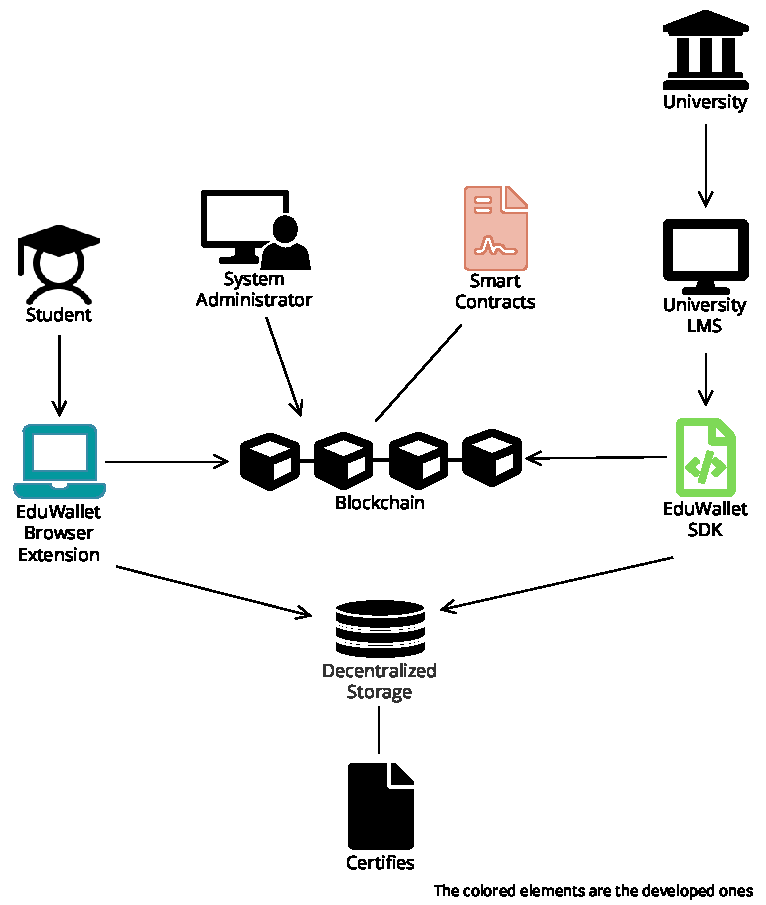
\includegraphics[width=0.6\textwidth]{figures/Architecture diagram basic.pdf}
  \caption[System basic architecture diagram]{Base architecture of the \acrlong{ew} system}
  \label{fig:baseArchDiag}
\end{figure}
In addition to these core components, we developed a simple yet complete \textbf{\acrfull{cli}}, which serves as a testing and demonstration tool and enables users to perform all operations typically available to universities, thereby simplifying the interaction with our \acrshort{sdk}. Because the focus of our work is on the interaction of universities and students with the academic registry, the system administrator's core functionalities\footnote{The approval and subscription of universities} have been inserted directly in the \acrshort{cli}. This design decision streamlines our use case and reduces unnecessary complexity.

The next chapters provide a detailed breakdown of the on-chain (\cref{chap:onchainDesign}) and off-chain (\cref{chap:offchainDesign}) designs.
\chapter{On-Chain Design}

\section{Blockchain Platform and Technologies}
The development of a blockchain-based system begins with the selections of a suitable blockchain platform. We selected \acrlong{eth}, a public blockchain known for its extensive developer community and rich ecosystem of features particularly suitable for an academic record systems \cite{mustafa2024publiceduchain}\cite{yassynzhanbolatzhan2021verificationuniversitystudent}. \acrlong{eth} supports smart contract development in multiple languages and serves as the foundation for various layer 2 solutions that enhance performance and scalability. This flexibility allows the system to be initially developed for the \acrlong{eth} mainnet and later migrated to a layer 2 chain to take advantage of specific features, with minimal development overhead. Notable \acrlong{eth}-based layer 2 solution include:

\begin{itemize}
    \item \textbf{Polygon}, offering faster and more cost-efficient transactions than the Ethereum mainnet.
    \item \textbf{Arbitrum}, improving scalability while maintaining compatibility with Ethereum smart contracts.
    \item \textbf{ZKsync}, ensuring high security and rapid finality through validity proofs.
    \item \textbf{Optimism}, emphasizing simplicity and seamless integration with the Ethereum ecosystem.
    \item \textbf{Starknet}, introducing its own high-performance language, Cairo\footnote{\url{https://www.cairo-lang.org/}}, optimized for zero-knowledge computation.
\end{itemize}

For the implementation, we selected Solidity\footnote{\url{https://soliditylang.org/}} as the programming language. Solidity is an object-oriented language, designed specifically for writing smart contracts on \acrlong{eth} and the \acrshort{evm}, influenced by C++, JavaScript and Python\footnote{\url{https://github.com/ethereum/solidity/blob/develop/docs/index.rst}}. It is the most widely adopted language in the \acrlong{eth} ecosystem, supported by and active and large developer community. Given our prior experience with Solidity, this choice was natural and well-suited to our objectives.

\section{Architecture}
\begin{figure}
  \centering
  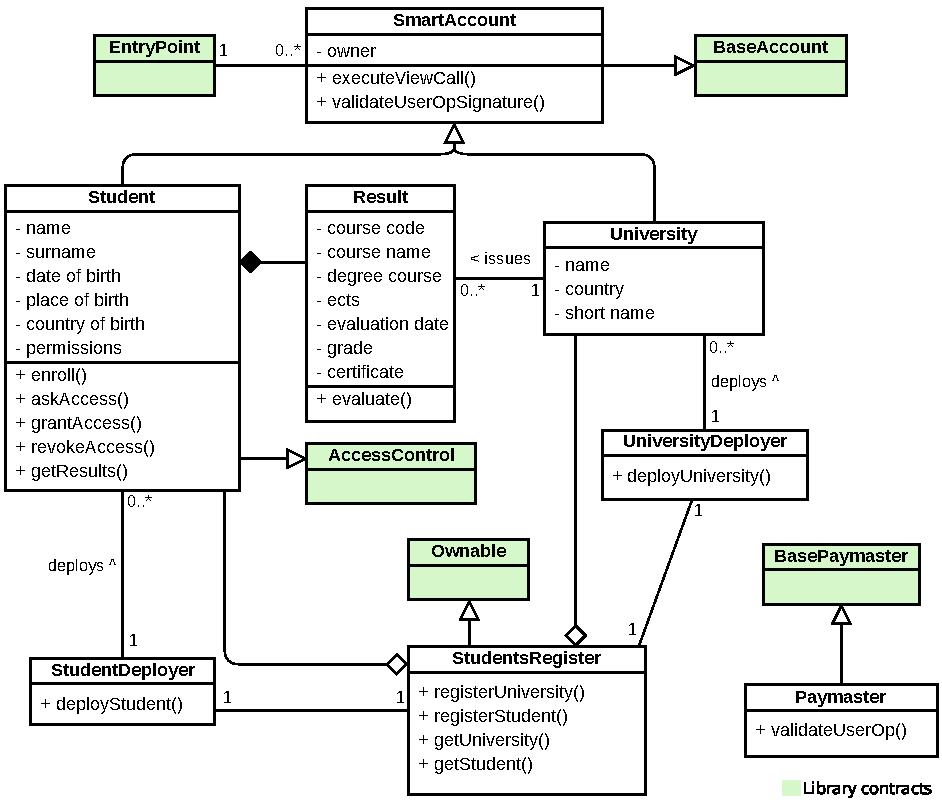
\includegraphics[width=1\textwidth]{figures/Contracts class diagram.pdf}
  \caption[Smart contracts architecture class diagram]{Class diagram representing smart contracts architecture}
  \label{fig:contractsClass}
\end{figure}

The overall architecture of the system is illustrated in the class diagram in \cref{fig:contractsClass}. The \acrshort{ew} system is composed of seven custom smart contracts, represented as white classes in the diagram. (\textit{Result} is not a smart contract, see \cref{ssec:studentContract} for more details). 

\begin{enumerate}
    \item \textbf{SmartAccount}: Defines the structure of a smart account following the account abstraction protocol.
    \item \textbf{Student}: Represents an individual student in the system.
    \item \textbf{University}: Represents a university entity.
    \item \textbf{StudentDeployer}: Responsible for deploying \textit{Student} contracts.
    \item \textbf{UniversityDeployer}: Deploys \textit{University} contracts.
    \item \textbf{StudentsRegister}: Manages and stores information about students and universities.
    \item \textbf{Paymaster}: Sponsors blockchain transactions made by students and universities.
\end{enumerate}
It addition, the system relies on four external contracts, shown in green in \cref{fig:contractsClass}, which are derived from established libraries such as \textit{OpenZeppelin}\footnote{https://openzeppelin.com/}:
\begin{enumerate}
    \item \textbf{EntryPoint}: A singleton contract that receives transactions from smart accounts and executes user operations.
    \item \textbf{AccessControl}\footnote{\url{https://docs.openzeppelin.com/contracts/5.x/access-control}}: Provides a comprehensive role-based access control mechanism.
    \item \textbf{BaseAccount}: Abstract contract defining the core behaviors of a smart account under the account abstraction protocol.
    \item \textbf{BasePaymaster}: Abstract contract defining the structure of a paymaster that sponsors user transactions.
\end{enumerate}

\subsection{SmartAccount}

\subsection{Student}
\label{ssec:studentContract}
The \textit{Student} contract encapsulates the majority of the system's logic. Its primary responsibilities include storing the student's personal information, such as name, surname, date of birth, place of birth and country of birth, as well as managing their academic records. These records are stored using the structure presented in \cref{lst:resultStruct}. 
\lstinputlisting[
    caption={\textit{Result} structure within the \textit{Student} smart contract},
    label=lst:resultStruct,
    language=Solidity,
]{listings/result.sol}
Due to Solidity's limited support for floating-point numbers, and because the \acrshort{ects} credits may not always be whole number, the \acrshort{ects} value is stored as the original number multiplied by 100. The type \textit{uint16} is used for this purpose, allowing values up to 655.36\footnote{The maximum number representable with 16 bits is 65536},  which is more than sufficient for academic credit systems. A smaller unsigned integer type, such as \textit{uint8}, supports only values from 0 to 2.55 in this context, which is clearly inadequate. The field \textit{certificateHash} stores the CID of the certificate, acting as a reference to its location in the decentralized storage system (see BACKGROUND\_IPFS and \cref{sec:decStorageDesgn} for further explanation). 

Additional functionalities, all addressing \textit{FR 5} in \cref{tab:funcReq}, include enabling universities to:
\begin{itemize}
    \item Retrieve a student's personal and academic information.
    \item Enrol the student in a new course.
    \item Record and evaluation for course the student has already attended.
\end{itemize}
All such interactions are governed by a strict access control mechanism, implemented to fulfill the relevant functional requirements outlined in \cref{tab:funcReq}, namely \textit{FR 6}, \textit{FR 7}, and \textit{FR 12}. This mechanism is based on the \textit{AccessControl} library, specifically the \textit{AccessControlEnumerable} variant, which enables the definition of roles and their association with specific addresses. Within the \textit{Student} contract, four distinct roles are defined:

\begin{enumerate}
    \item \textbf{reader}
    \item \textbf{writer}
    \item \textbf{reader requester}
    \item \textbf{writer requester}
\end{enumerate}
These roles cover all possible scenarios. When an institution requests read or write access to a student's academic records,  its smart account address is assigned the corresponding role. Since \textit{AccessControlEnumerate} supports enumeration of role bearers, the student can query and view which institutions have pending access requests. When an institution attempts to access or modify a student's academic records, the \textit{Student} contract verifies whether the caller's address has been granted the appropriate role, thereby enforcing access restrictions. This mechanism requires the \textit{Student} contract to support a set of permission management functions, including the ability for students to grant, revoke, and inspect permissions (\textit{FR 12}), as well as for universities to request and verify their access rights (\textit{FR 7}).

As shown in \cref{fig:useCaseCli}, \textit{Student} contracts are deployed by the \textit{StudentDeployer}, which is invoked by the \textit{StudentsRegister} contract when a university registers a new student in the \acrshort{ew} system. Upon registration, the initiating university is automatically granted write permissions for the student's academic record, reflecting its role as the enrolling institution responsible for issuing evaluations. All subsequent interactions with the \textit{Student} contract are carried out either by the browser extension or the \acrshort{sdk}. The browser extension is responsible for retrieving personal and academic data and managing permissions on the student's behalf. The \acrshort{sdk}, on the other hand, acts on behalf of universities to access and modify the student's academic wallet. To facilitate these interactions, the \textit{Strudent} contract defines several structured data types, which are used for functions inputs and outputs. These structures improve code readability and usability by grouping related data into cohesive types. Instead of requiring users to  pass multiple separate parameters in a specific order, an approach that increases the risk of errors, developers can simply import the relevant structure and populate its fields. The data type defined in the \textit{Student} contract are:

\begin{itemize}
    \item \textbf{EnrollmentInfo}: Contains the information required to enrol a student in a course; used as input for the enrolment function.
    \item \textbf{EvaluationInfo}: Contains the data needed to record an evaluation; used as input for the evaluation function.
    \item \textbf{Result}: Previously presented, this structure stores the details of a course attended by the student and is used to return the student's academic records.
    \item \textbf{StudentBasicInfo}: Represents the student's personal information.
    \item \textbf{StudentInfo}: A composite structure that includes the \textit{StudentBasicInfo} and a list of \textit{Result} structures, representing the student’s complete academic profile.
\end{itemize}

\subsection{University}
Since the primary focus of this work is on the interaction between students and their academic records, as well as the ownership of such data, the institutional accounts (smart accounts) of universities, implemented through the \textit{University} contract, are designed to simpler that those of students. The \textit{University} contract, like \textit{Student}, extends the \textit{BaseAccount} contract, enabling it to function as a smart account compatible with the account abstraction protocol. As a result, universities can use their institutional wallet, via the \acrshort{sdk}, to perform blockchain transactions, which are then sponsored by the \textit{Paymaster}. 

In addition, because universities are identified solely by their contract address in interactions with other smart contracts, the \textit{University} contract also stores descriptive metadata, including the institution's name, country, and a short identifier. Apart from the \textit{UniversityDeployer}, which is responsible for deploying the contract, the only components that interact directly with the \textit{University} contract are the \acrshort{sdk} and the browser extension. When these components need to access university-related information, they do so using the institution's contract address. For instance, when a student retrieves their academic records, each record references the issuing university by it address. The browser extension must then query the blockchain to access the corresponding \textit{University} contract and extract the relevant metadata.    

\subsection{StudentDeployer and UniversityDeployer}
The deployment of \textit{Student} and \textit{University} contracts is handled by the \textit{StudentDeployer} and \textit{UniversityDeployer} contracts, respectively. When a system administrator registers a new university, or a university registers a new student through the \acrshort{sdk}, they interact with the \textit{StudentsRegister} smart contract. This contract, in turn, invokes one of the deployer contracts to create the corresponding smart contract instance. This architecture implements the factory pattern, a design principle commonly used in object-oriented programming to abstract the creation of objects. In the context of the \acrshort{ew} system, the deployer contracts abstract and encapsulate the instantiation of new \textit{Student} and \textit{University} contracts.

The adoption of the factory pattern offers several advantages over embedding the deployment logic directly within the \textit{StudentsRegister} contract:

\begin{itemize}
    \item It separates the contract creation logic from the registration logic, improving modularity and maintainability.
    \item It reduces the complexity of the \textit{StudentsRegister} contract by externalizing the deployment process.
    \item It minimizes the contract size of \textit{StudentsRegister}. In Solidity, deploying a contract via the \texttt{new} keyword requires embedding the bytecode of the deployed contract, which increases the size of the calling contract. Since Solidity enforces a maximum contract size of 24576 bytes, including large deployment code directly could exceed this limit. Using external deployer contracts bypass this issue.
\end{itemize}

The decision to centralize deployments through the \textit{StudentsRegister} contract was also motivated by gas efficiency. On blockchain platforms, reducing the number of transactions typically leads to lower gas costs. By combining the deployment of a contract and the registration of its address into a single transaction, the system reduces the overall gas consumption required for onboarding new entities.

\subsection{StudentsRegister}

\subsection{Paymaster}
One of the system's key feature is that blockchain usage is nearly transparent for users. Students do not directly interact with wallets or perform transactions themselves, and universities only need the private key associated with their \acrshort{eth} account to manage their institutional smart wallet. This level of abstraction is made possible by the \textit{Paymaster}, a smart contract deployed on the blockchain that sponsors all transactions made by users. This design directly readdressing \textit{NFR 5} (see \cref{tab:nonFuncReq}), which emphasizes minimizing the complexity of interactions with the system for end users.

Without the \textit{Paymaster}, the system would require a mechanism to fund user wallets, presenting three primary options:

\begin{enumerate}
    \item Each user funds their own wallet.
    \item Universities fund the wallets of both students and themselves.
    \item The \acrshort{ew} system centrally manages and funds all wallets.
\end{enumerate}
Each approach has significant drawbacks. The first and second require users to manage cryptocurrency wallets and purchase tokens, which increases complexity and cost, especially burdensome for students. The third alternative still introduces administrative overhead and security concerns related to managing a large number of wallets.

Our solution utilizes a \textit{Paymaster} that implements the \textit{BasePaymaster} abstract contract, developed as part of the ERC-4337 protocol\footnote{\url{https://www.erc4337.io/}}. For simplicity, our current implementation sponsors all user operations (transactions) it receives, without validating their origin or gas cost. The only enforced constraint, inherited from \textit{BasePaymaster}, is that transactions must be routed through a known \textit{EntryPoint} contract.
This configuration is suitable for testing environments such as local or test networks, where there is no risk of losing real tokens. In a real-world deployment, a more robust implementation would be necessary, specifically, one that integrates with the \textit{StudentsRegister} contract to verify that the transaction sender is a verified student or university. 
\chapter{Off-Chain Design}
\label{chap:offchainDesign}
In this chapter, we present the design of the of-chain components of the \acrlong{ew} environment, which have been developed to offer a user-friendly interface for stakeholders and support the integration of system functionalities. Together with the smart contracts described in \cref{chap:onchainDesign}, these components form the complete system architecture, as illustrated in \cref{fig:fullArchDiag}. 

\begin{figure}[htpb]
  \centering
  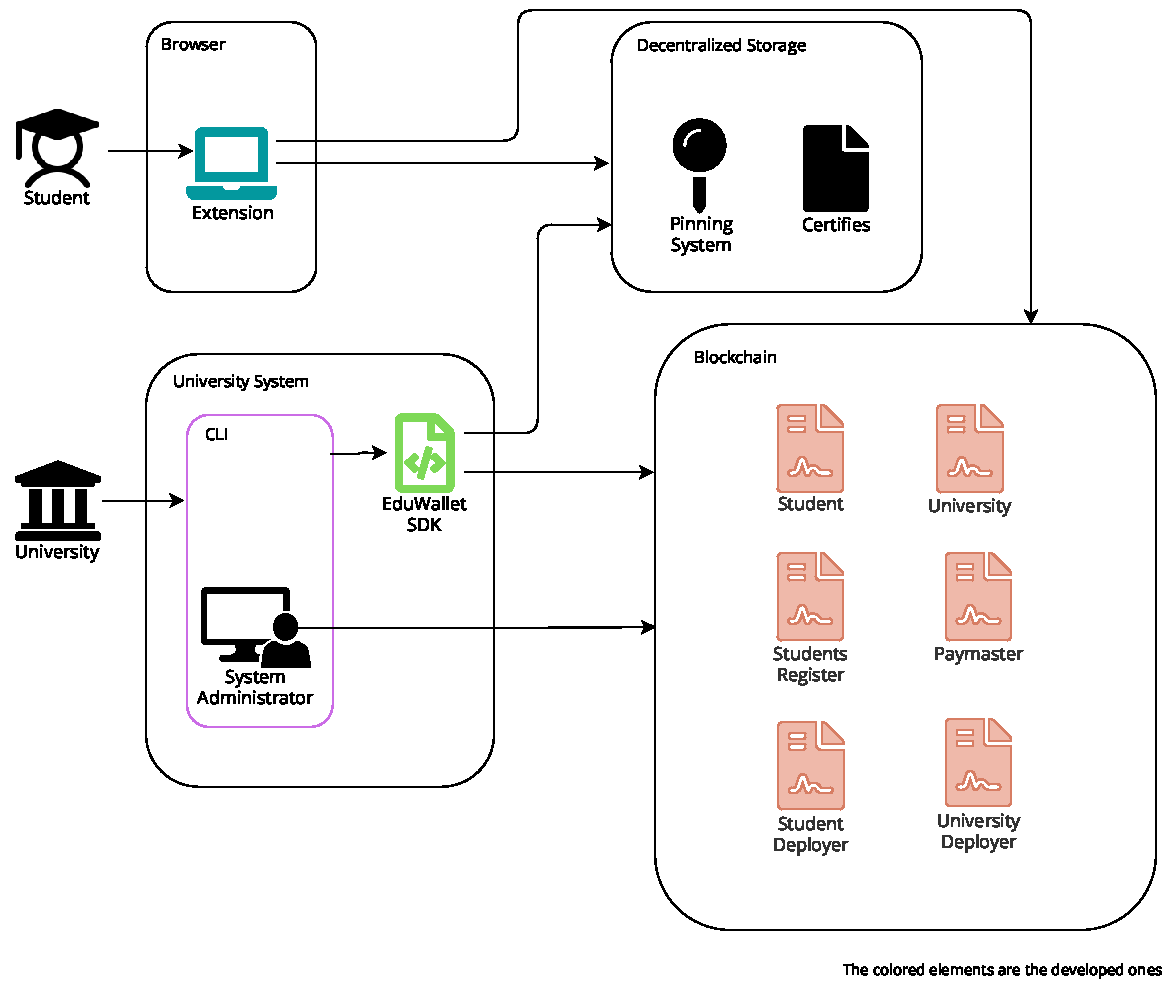
\includegraphics[width=0.8\textwidth]{figures/Architecture diagram complete.pdf}
  \caption[System architecture diagram]{Complete architecture of the \acrlong{ew} system}
  \label{fig:fullArchDiag}
\end{figure}

Given that students using \acrshort{ew} are not expected to have expertise in blockchain technologies, the platform must provide a simple yet effective interface. This interface should enable them to interact with their academic wallets, retrieve academic results, and manage access permissions. These requirements are address \textit{FR 11} in \cref{tab:funcReq}. Similarly, smart contracts interactions may pose challenges even for universities and their \acrfull{it} departments. Therefore, the system must also offer a simplified and accessible interface for institutional use, as specified in \textit{FR 8} in \cref{tab:funcReq}. 
To satisfy these usability needs, two primary components were developed: a \textbf{browser extension} for student interactions with their academic wallets, and a \textbf{\acrlong{sdk}} designed to facilitate the integration of \acrshort{ew} within university systems.

Moreover, \textit{NFR 3} in \cref{tab:nonFuncReq} emphasizes the need to minimize on-chain storage consumption and associated costs by limiting blockchain use to essential data only. To support this goal, the system incorporates a \textbf{decentralized storage} solution, which is responsible for storing and providing access to large data files, such as academic certificates and other supporting documentation.

Finally, to enable comprehensive testing of the environment, a \textbf{\acrlong{cli}} was developed. This tool simulates a real university \acrshort{lms} and allows for testing the \acrshort{sdk} functionalities, as well as its interaction with smart contracts and the decentralized storage layer.

%%%%%%%%%%%%%%%%%%%%%%%%%%%%%%%%%%%%%%%%%%%%%%%%%%%%%%%%%%%%%%%%%%
% BROWSER EXTENSION
%%%%%%%%%%%%%%%%%%%%%%%%%%%%%%%%%%%%%%%%%%%%%%%%%%%%%%%%%%%%%%%%%%
 \section{Browser Extension}
\label{sec:browserExtensionDesign}
This section presents the browser extension, which serves as the primary interface for students to interact with their academic wallets. Its main objective is to abstract the complexity of on-chain operations by offering a user-friendly interface that aligns with the design and usability standards of traditional web applications, addressing \textit{FR 11} in \cref{tab:funcReq}.

\subsection{Technological Choices}
To achieve the highest level of decentralization and autonomy for users, we chose to implement a browser extension rather than a traditional web application. Conventional web applications, typically accessed via a \acrshort{url}, rely on a server to host both the user interface (front-end) and the business logic (back-end), but this architecture introduces central points of control and potential failure. Such reliance would conflict with \textit{NFR 6} in \cref{tab:nonFuncReq}, which emphasizes the importance of minimizing centralization within the system's design.
In contrast, a browser extension operates more like a lightweight desktop application, but within the browser environment. This eliminates the need for an external server to host the interface and, since the core logic of the \acrlong{ew} system resides in smart contracts deployed on the blockchain, no additional server-side back-end is required. This architecture ensures that both the user interface and the underlying logic remain fully decentralized, depending only on the local extension and on-chain infrastructure.
Beyond decentralization, browser extensions offer a compact, wallet-like user experience. Rather than a full screen web page, they present a small, easily accessible window via an icon in the browser toolbar. This interaction model is common among cryptocurrency wallets, such as MetaMask, offering users an intuitive means of managing on-chain assets. Adopting the same paradigm for academic records helps students access and control their data seamlessly, reinforcing the concept on an academic wallet.

Browser extensions are supported across several major browsers, including Microsoft Edge, Google Chrome and Firefox. While each browser introduces minor platform-specific differences, we opted to develop the extension primarily for Google Chrome. Chrome currently holds the largest global browser market share\footnote{\url{https://en.wikipedia.org/wiki/Usage_share_of_web_browsers}}, offering a broad potential user base. Additionally, since Google Chrome and Microsoft Edge are both based on the Chromium open-source project, extensions developed for Chrome are also compatible with Microsoft Edge, further extending platform reach without additional development overhead.

Among the various technologies available for browser extensions development, we selected TypeScript as the core programming language and React as the framework for building the user interface. TypeScript offers the flexibility and web-centric capabilities of JavaScript while introducing static typing, which improves code safety, clarity, and maintainability. It also integrates seamlessly with smart contract development, as libraries exist to generate TypeScript types directly from contract definitions.
React, originally developed by Facebook as an open-source JavaScript library, is widely used for building modern web interfaces. It enables efficient \acrshort{ui} development and facilitates seamless interaction with application logic.
Our familiarity and prior experience with both React and JavaScript also influenced our choice, enabling a faster and more reliable development process. Additionally, we employed \textit{Vite} as the building tool for our environment, making it easier to manage and bundle the various modules of our browser extension efficiently.

\subsection{Functionalities}
\label{ssec:extFunctionalities}
The browser extensions provides students with all necessary tools to access and manage their academic wallets. The primary entry point is the login functionality. To authenticate, students enter the credentials (see \cref{fig:loginExtDesign}) supplied by the university at wallet creation. During login, the extension derives the private key of an \acrshort{eoa} from the student's ID and password using the PBKDF2 algorithm. PBKDF2 is a key-derivation function that, given a \gls{salt} and a password, produces the private key of an \acrlong{eth} \acrlong{eoa}. In our implementation, the student's ID serves as the \gls{salt}, eliminating the need for a centralized \gls{salt} repository and ensuring uniqueness per users. Upon deriving the private key and instantiating the \acrlong{eoa}, the extension queries the StudentsRegister contract to retrieve the associated \acrlong{sca} address. If a valid address is returned, authentication succeeds and the extension proceeds to fetch the student's personal details and academic records from their smart account.

\begin{figure}
  \centering
  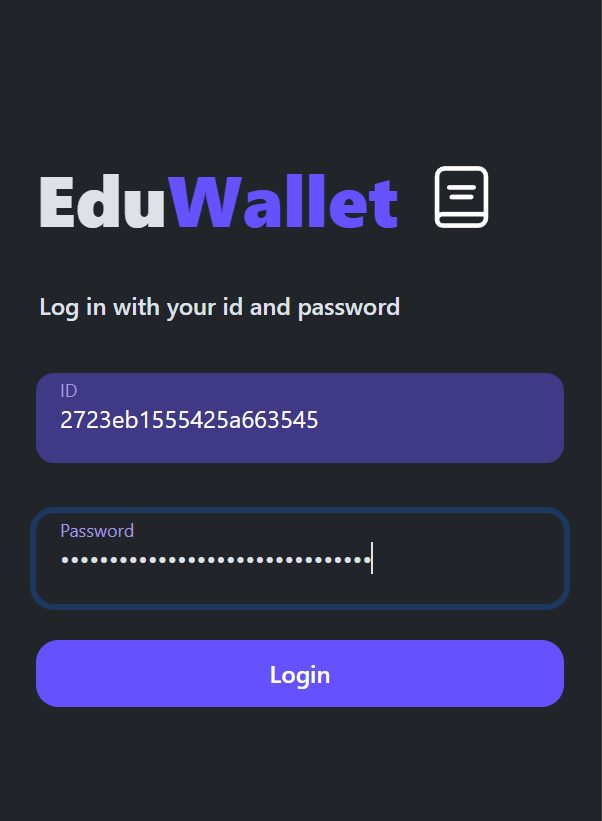
\includegraphics[width=0.45\textwidth]{figures/Login.png}
  \caption[Browser extension login page]{Screenshot of the browser extension login window.}
  \label{fig:loginExtDesign}
\end{figure}

Once logged in, students can view a consolidated list of their academic records (\cref{sfig:homepageExt}) and inspect individual entries (\cref{sfig:singleRecordExt}). Records are grouped first by university, using each institution's short identifier, and then by degree program. Each entry displays the course name, course code, \acrshort{ects} credits, and grade, if available. The homepage also shows the student's total accumulated \acrshort{ects}. Selecting a record opens its detailed view, which adds the date of evaluation and hyperlink to the certificate stored on the decentralized storage system. 

\begin{figure}
    \centering
    \begin{subfigure}{.45\textwidth}
        \centering
        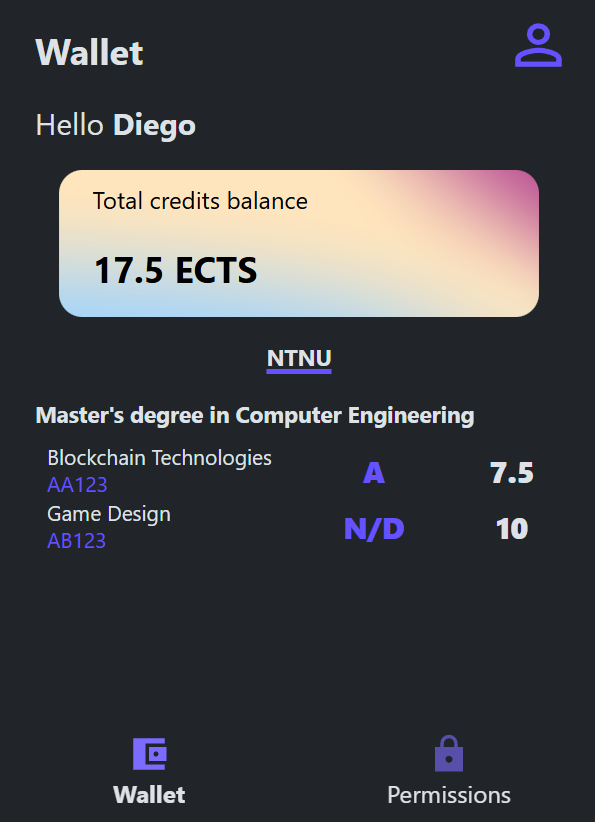
\includegraphics[width=\textwidth]{figures/Homepage.png}
        \caption{Homepage}
        \label{sfig:homepageExt}
    \end{subfigure}
    \hfill
    \begin{subfigure}{.45\textwidth}
        \centering
        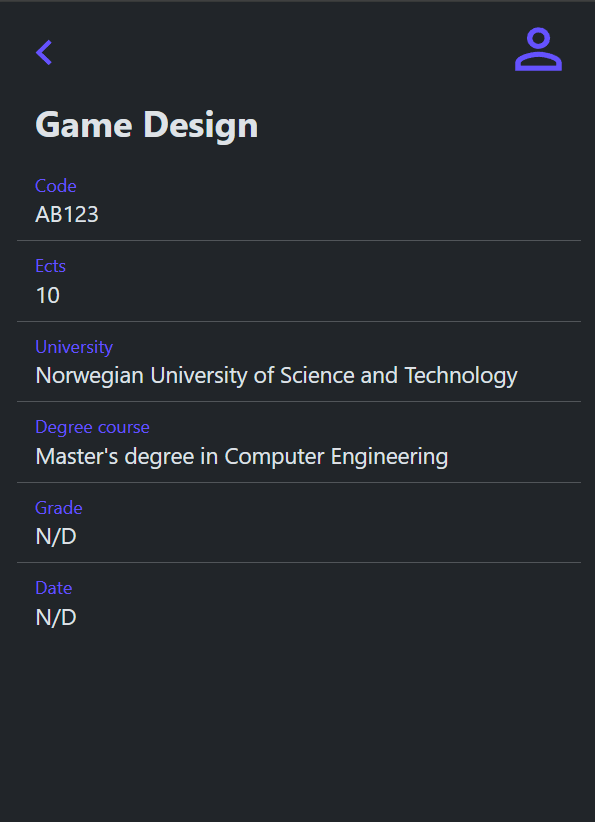
\includegraphics[width=\textwidth]{figures/SingleCourse.png}
        \caption{Single record page}
        \label{sfig:singleRecordExt}
    \end{subfigure}
    \caption[Browser extension windows for academical records]{Screenshots of the browser extension showing the academic records homepage and detailed record view.}
    \label{fig:recordsExt}
\end{figure}

The extension also supports permission management via the lock icon. In this interface (\cref{fig:permissionsExt}), students can review granted permission and pending access requests from universities. The permissions are categorized into three groups: requests, read permissions and the write permissions. Buttons adjacent to each entry enable students to easily grant new permissions or revoke existing ones, ensuring full control over their academic wallet.

\begin{figure}
  \centering
  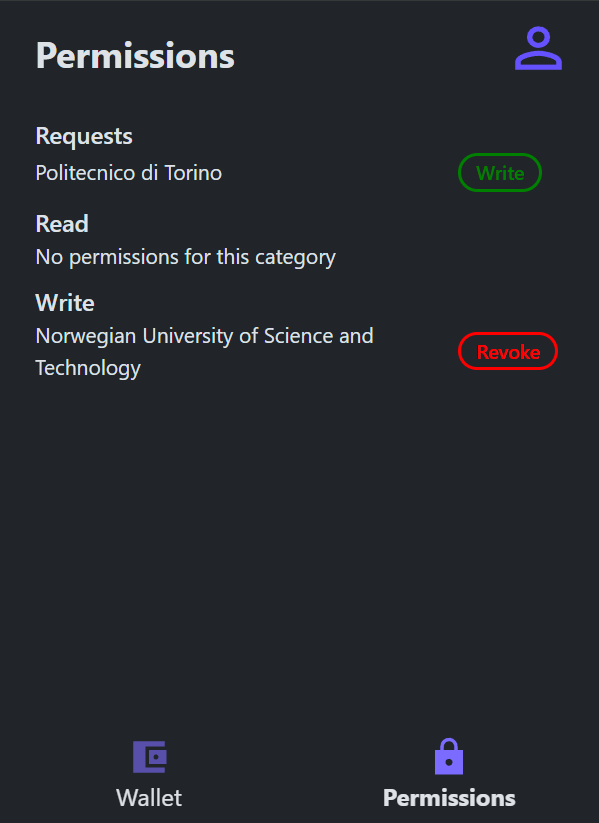
\includegraphics[width=0.45\textwidth]{figures/Permissions.png}
  \caption[Browser extension permissions page]{Screenshot of the extension permissions window.}
  \label{fig:permissionsExt}
\end{figure}

Finally, clicking the user icon in the top‐right corner opens the personal information page, where students can view their profile details (\cref{fig:userInfoExt}).

\begin{figure}
  \centering
  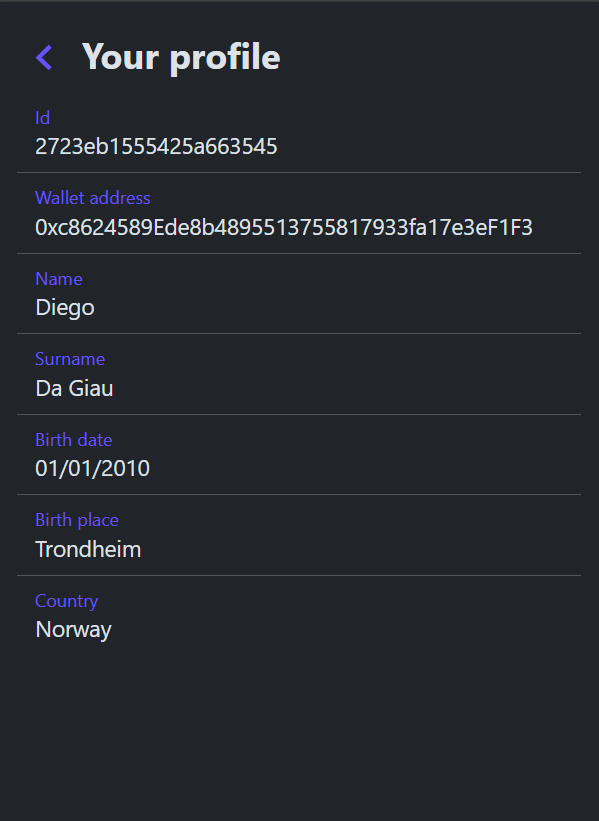
\includegraphics[width=0.45\textwidth]{figures/PersonalInfo.png}
  \caption[Browser extension user information page]{Screenshot of the browser extension user information window.}
  \label{fig:userInfoExt}
\end{figure}

\subsection{Blockchain Interactions}
\label{ssec:extBlockchainInteraction}
The most straightforward way to perform on-chain operations from off-chain components is by using external libraries specifically designed to streamline these interactions. The two primary options are \textit{web3}\footnote{\url{https://web3js.readthedocs.io/en/v1.10.0/index.html}} and \textit{ethers}\footnote{\url{https://docs.ethers.org/v6/}}. We opted for \textit{ethers} over \textit{web3} because it is more lightweight, an essential feature for web applications that must minimize browser resource usage, and because it is more modern and offers better TypeScript support. 
Another crucial library used in the development of the extension is \textit{TypeChain}, a TypeScript-oriented tool that, given the Solidity code of smart contracts, extracts type definitions that can be imported directly into the application. This ensures our application remains type-safe and consistent with the structures and requirements defined in the smart contracts that comprise \acrlong{ew}. 

With these libraries in place, the browser extension needs to establish a connection to the blockchain to execute operations. Our system leverages the \textit{ethers} JSON-RPC provider, which connects to a chain via its \acrshort{url}. The \acrshort{url} of the used chain is hardcoded in the extension, along with the addresses of the core contracts, namely, the StudentsRegister, EntryPoint and Paymaster (see \cref{lst:confExt}). To deploy the extension on a different configuration, such as a layer 2 network with a new \acrshort{url} and different core contract addresses, these values must be manually updated in the extension's source code.

\lstinputlisting[
    caption={Blockchain configuration info data variable and its type definition},
    label=lst:confExt,
    language=TypeScript
]{listings/conf.ts}

To support the required on-chain functionalities, the browser extension performs three types of interactions:
\begin{enumerate}
    \item Direct read-only operations
    \item Read-only operations via the \acrlong{sca}
    \item Transactions via the smart account
\end{enumerate}

\subsubsection{Direct Read-Only Operation}
This is the simplest interaction and is executed, for example, during login phase, where the extension retrieves the address of the student's smart account. In this case, the extension directly invokes the corresponding function of the StudentsRegister contract, using the student's \acrshort{eoa} as the sender. 

\subsubsection{Read-Only Operation via Smart Account}
These interactions occur when retrieving permissioned data, such as academic records, accessible only to authorized universities or the student. For this, the extension invokes the dedicated function to execute read-only operations, provided by the SmartAccount contract. As described in \cref{sec:smartAccountDesign}, the call requires specifying:

\begin{itemize}
    \item the address of the target contract
    \item the encoded function signature and parameters (call data)
\end{itemize}
Encoding is handled using functions from the \textit{ethers} library. The operation is executed using the student's \acrshort{eoa}.

\subsubsection{Transaction via Smart Account}
This type of interaction is required for operations that alter blockchain state, such as granting or revoking permissions to universities, by accessing restricted functions. These actions require gas consuming transaction executed via the student's \acrlong{sca}, using UserOperations.
The browser extension constructs a UserOperation by assembling the following fields:
\begin{itemize}
    \item Sender address (the student's \acrshort{eoa} address)
    \item Target contract address
    \item Encoded function name and parameters
    \item Gas and fee-related parameters
    \item Transferred value (always set to 0 in our case)
    \item Paymaster address and associated parameters
    \item Student's \acrshort{eoa} signature, generated using \textit{ethers} utilities
\end{itemize}
After constructing the UserOperation, the extension sends it directly to the EntryPoint contract using its hardcoded address. As discussed in \cref{ssec:accountAbstraction}, in a public network deployment, this operation would be relayed via a bundler instead.

\subsection{UI Prototyping}
The \acrlong{ui} was initially designed using \textit{Figma}, a powerful prototyping tool that enables detailed visualization and planning \acrlong{ui} across various types of applications. The \acrshort{ui} prototype, accessible via the link provided in \cref{chap:figma}, played a crucial role not only in shaping the visual layout of the extension, but also in refining its functional requirements. 
By sketching out all application windows and placing ourselves in the shoes of end users, we were able to identify the key pieces of information the interface needed to convey and determine the most effective ways to present them. 

%%%%%%%%%%%%%%%%%%%%%%%%%%%%%%%%%%%%%%%%%%%%%%%%%%%%%%%%%%%%%%%%%%
% SDK
%%%%%%%%%%%%%%%%%%%%%%%%%%%%%%%%%%%%%%%%%%%%%%%%%%%%%%%%%%%%%%%%%%
\section{Software Development Kit}
\label{sec:sdkDesign}
This section describes the \acrlong{sdk}, a TypeScript package designed to simplify integration of the \acrlong{ew} system within university infrastructure. By abstracting low-level blockchain concerns, such as \acrshort{eoa} key management, contract deployment and referencing, read-only queries and gas consuming transactions, the \acrshort{sdk} lowers the barrier to entry for institutions wishing to adopt on-chain academic records.

When evaluating integration strategies, we considered two alternatives: web \acrshort{api}s and a stand-alone \acrshort{sdk}. Web \acrshort{api}s require a centralized server to receive client requests, execute business logic, and relay blockchain interactions. In contrast, an \acrshort{sdk} is distributed as a client-side library that runs directly within the user's environment, requiring no dedicated server infrastructure beyond standard package hosting. This approach aligns with \textit{NFR 6} in \cref{tab:nonFuncReq}, which prioritizes decentralization.
Moreover, an \acrshort{sdk} offers superior scalability compared to \acrshort{api}s. Since \acrshort{api} calls traverse the public internet and share server resources, they can be affected by network latency or server overload when serving thousands of institutions worldwide. The \acrshort{sdk}, by running locally on each institution's system, minimizes network dependencies and leverages the user's own compute resources.
However, \acrshort{sdk}s entail two main trade-offs. First, updates depend on consumer upgrading to newer package versions, whereas a centralized \acrshort{api} can be improved transparently. Second, \acrshort{sdk}s are inherently platform-specific: a TypeScript \acrshort{sdk} supports only JavaScript/TypeScript environments. To address this, one must develop and maintain multiple \acrshort{sdk} variants for different languages or platform.

Given that our off-chain components are implemented in TypeScript, and that Node.js\footnote{An open-source server environment used to run JavaScript and TypeScript code outside the browser (\url{https://nodejs.org})} is widely adopted in modern back-end systems, we selected TypeScript for the \acrshort{sdk}. The choice maximizes compatibility with university \acrshort{it} stacks and leverages existing expertise in the JavaScript ecosystem.

\subsection{Working with the SDK}
Once imported in the university's system, the \acrshort{sdk} exposes a suite of functions and types that encapsulate all interaction with the on-chain academic record platform. An example of its usage is shown in \cref{lst:sdkCall}, where the \acrshort{sdk} is imported and used to register a student in the system. The registration function accepts two parameters: the university \acrshort{eoa} wallet, instantiated from the private key provided at university enrolment using the \textit{ethers} \texttt{Wallet} type; and a \texttt{StudentData} object, a type defined by the SDK that includes the student’s name, surname, date of birth (YYYY-MM-DD), place of birth, and country of birth. The function returns the student's credentials (ID and password) and the \acrshort{sca} address. Because all \acrshort{sdk} calls involve blockchain queries or transactions, each function is declared asynchronous and must be awaited by the caller.

\lstinputlisting[
    caption={Import of the \acrshort{sdk} and exemplar invoke},
    label=lst:sdkCall,
    language=TypeScript
]{listings/sdkCall.ts}

In addition to students registration, the \acrshort{sdk} provides the following core functionalities for university integrators:
\begin{itemize}
    \item Enrol a student in one or more courses.
    \item Record a new evaluation for a student.
    \item Retrieve a student’s personal details.
    \item Retrieve a student’s personal details and complete academic records.
    \item Request permission to read from or write to a student’s academic wallet.
    \item Verify an existing permission in a student’s academic wallet.
\end{itemize}

\subsubsection{Register a student}
Universities register students by providing their own \acrshort{eoa} and a \texttt{StudentData} object. The \acrshort{sdk} generates a new \acrshort{eoa} for the student using PBKDF2 algorithm, already presented in \cref{ssec:extFunctionalities}. Specifically, the \acrshort{sdk} randomly generates a student's ID and password, which are used as inputs to derive the private key. This approach satisfies \textit{NFR 1} in \cref{tab:nonFuncReq} by avoiding reliance on third-party wallets (e.g., MetaMask). The \acrshort{sdk} then constructs a UserOperation to invoke the registration function on the StudentsRegister contract via the university's smart account. Finally, it queries the StudentsRegister to retrieve the student's \acrshort{sca} address and returns it, along with the student's credentials, to the caller.

\subsubsection{Enrol a student}
To enrol students in courses, the \acrshort{sdk} requires the university's \acrshort{eoa} wallet, the student's \acrshort{sca} address, and an array of \texttt{CourseInfo} objects, each containing course code, name, degree program, and \acrshort{ects} credits. The \acrshort{sdk} converts these into the format expected by the Student contract's \texttt{Result} structure (\cref{sec:studentContract}) and submits a UserOperation to perform the enrolment.

\subsubsection{Record a new evaluation}
Recording an evaluation requires the university’s \acrshort{eoa} wallet, the student’s \acrshort{sca} address, and an array of \texttt{Evaluation} objects. Each object includes the course ID, grade, evaluation date, and an optional path to a certificate file. For entries that include certificates, the \acrshort{sdk} first uploads the file to the decentralized storage system (see \cref{sec:decStorageDesgn}) and retrieves a reference to it. It then assembles a UserOperation containing all relevant data, including the storage reference. This UserOperation is executed via the university's smart account to invoke the evaluation function in the student's \acrshort{sca}.

\subsubsection{Retrieve Student Details and Records}
To fetch personal details, with or without academic records, the \acrshort{sdk} takes the university's \acrshort{eoa} wallet and the student's \acrshort{sca} address. It executes a read-only operation via the university's \acrshort{sca}, to invoke the appropriate view function on the student's smart account. Upon success, the \acrshort{sdk} maps the returned data into a \texttt{Student} object, containing \texttt{StudentData} and an array of academic records.

\subsubsection{Request a permission}
When a university needs permission to read or write a student’s academic wallet, the SDK requires the university’s \acrshort{eoa} wallet, the student’s \acrshort{sca} address, and the desired permission type (\texttt{Read} or \texttt{Write}). It then constructs and submits a UserOperation to call the corresponding function on the student’s \acrshort{sca}.

\subsubsection{Verify permissions}
To verify existing permissions, the \acrshort{sdk} takes the university's \acrshort{eoa} wallet and the student's \acrshort{sca} address. It then executes a read-only operation via the university's smart account, targeting the student smart account. The student's \acrshort{sca} returns the granted permission type, or null if none is held. The \acrshort{sdk} forwards this result to the caller, using the appropriate TypeScript type.

\subsection{Access On-Chain Functionalities}
Since the \acrshort{sdk} adopts the same model as the browser extension to access on-chain functionalities, the \cref{ssec:extBlockchainInteraction} provides a thorough explanation of the different types of interactions, as well as the tools and libraries used to execute them.

\subsection{Input Management}
All the \acrshort{sdk} functions perform input validation and presence check to ensure data integrity. For instance, the function responsible fro registering a new evaluation in a student's academic wallet first verifies that all requires parameters are provided. It then checks whether the student's smart account address is valid by confirming it begins with '0x'. This function also ensures that the array of evaluations contains at least one entry and, for each evaluation, verifies the presence of all mandatory fields.

%%%%%%%%%%%%%%%%%%%%%%%%%%%%%%%%%%%%%%%%%%%%%%%%%%%%%%%%%%%%%%%%%%
% DECENTRALIZED STORAGE SYSTEM
%%%%%%%%%%%%%%%%%%%%%%%%%%%%%%%%%%%%%%%%%%%%%%%%%%%%%%%%%%%%%%%%%%
\section{Decentralized Storage System}
\label{sec:decStorageDesgn}
This section presents our solution to one of the most significant challenges in blockchain-based systems: the high cost of on-chain storage. To address this issue, presented also through the \textit{NFR 3} in \cref{tab:nonFuncReq}, we introduce an off-chain decentralized storage solution in our project. This system is used to store and retrieve certification files, such as language certificates or graduation diplomas, which require significantly more space than plain text\footnote{PDF files typically range from a few kilobytes to several megabytes, whereas plain text data usually occupies only a few bytes.}. Storing such documents directly on-chain would result in substantial gas costs, making the approach impractical. 

We chose a decentralized storage system over traditional local or cloud-based solutions to maintain the decentralized nature of our environment and to meet \textit{NFR 6} outlined in \cref{tab:nonFuncReq}. Among the various decentralized options available, we selected \acrfull{ipfs} for its ability to provide verifiable and distributed file storage. This choice is motivated by several factors: \acrshort{ipfs} is an open source protocol with a large and active community, strong support, and widespread adoption. It also serves as the foundational layer for many other decentralized platforms, such as Filecoin\footnote{\url{https://filecoin.io}} and Web3.Storage\footnote{\url{https://web3.storage}}, allowing future extensions or upgrades to be implemented with minimal effort \cite{erikflorian2022ipfsandfrineds}. Furthermore, \acrshort{ipfs} ensures immutability of stored files, a critical feature for academic certificates, which must remain unchanged over time.

\subsection{Pinning files}
To fully leverage \acrshort{ipfs}, we integrated Filebase\footnote{\url{https://filebase.com}}, a third-party pinning service. Pinning refers to the act of instructing a node to keep a copy of a file permanently, preventing it from being removed during garbage collection. Without Filebase, we would have needed to run our own local \acrshort{ipfs} node and manage file pinning manually, an approach that introduces instead complexity, higher maintenance costs, and reduced data availability in a testing system like ours. In contrast, Filebase handles node operation and file pinning, offering an accessible solution thorough its AWS S3-compatible \acrshort{api}, which simplifies file uploads to the peer-to-peer network. Notably, Filebase also provides a free tier allowing up to 5 GB of storage, which is sufficient for our needs. This is an advantage over other pinning solutions such as Web3.Storage, which lacks a fully free plan, or Pinata\footnote{\url{https://pinata.cloud}}, which offers more limited options.

\subsection{Integration in the system}
As illustated in \cref{fig:fullArchDiag}, both the browser extension and the \acrshort{sdk} interact with the storage system. The browser extension enables students to retrieve certificates associated with their academic records through the official \acrshort{ipfs} public gateway. As shown in \cref{fig:courseWithCertificate}, each certificate is presented as clickable, composed by the gateway's base \acrshort{url} followed by the file's \acrfull{cid} on the \acrshort{ipfs} network. The \acrshort{cid} of each document is stored on-chain within the student's academic wallet, alongside other record information such as the course name (see \cref{sec:studentContract}). This enables students to view and download their certificates from a standard web interface.

\begin{figure}
  \centering
  
\includegraphics[width=0.45\textwidth]{figures/SingleCourseWithCertificate.png}
  \caption[Browser extension screenshot with certificate link]{Screenshot of the browser extension presenting the page of a course. The image shows the link to the certificate saved in the decentralized storage.}
  \label{fig:courseWithCertificate}
\end{figure}

Similarly, the \acrshort{sdk} uses the same mechanism to retrieve certificates on behalf of universities. When uploading a file, however, the \acrshort{sdk} interacts directly with Filebase to ensure the file is pinned and hosted by an active node. The \acrshort{sdk} receives the document from the university, then uses the AWS S3-compatible \acrshort{api} to upload it. The \acrshort{api} requires the key associated with the pinning account (managed by the \acrshort{ew} system administrator) and the file itself. In return, it provides the \acrshort{cid}, which is then stored in the academic record.
% TODO: Reference implementation section

\subsection{Security and Limitations}
Academic certifies, and official documents more broadly, are legal artifacts that must always be secure and verifiable. \acrshort{ipfs} inherently supports these properties through its use of content-based addressing. In this model, each file is identified by a \acrshort{cid}, which is derived from the cryptographic hash of the file's content. Any alteration to the file results in a completely different \acrshort{cid}, ensuring that tampering is immediately detectable \cite{benet2014ipfscontentaddressed}. Since the \acrshort{cid} is stored on the blockchain at the time the certificate is issued by the university, the document's authenticity and integrity are guaranteed.

While \acrshort{ipfs} offers strong immutability and verifiability, it lacks built-in access control. In the context of our system, we assume that certificates are publicly accessible documents. Consequently, any part in possession of a file's \acrshort{cid} can retrieve it via the public gateway. However, if access control becomes a requirement, there are several strategies to address this limitation \cite{barbaraanrealaura2021datapersistence}. One option is to encrypt files before uploading them to \acrshort{ipfs}, such that only authorized components within our system can decrypt them. Another approach is to use a private \acrshort{ipfs} network, where access can be restricted to approved entities. The trade-offs and potential implications of such private deployment will be discussed in the FUTURE\_WORK\_REFERENCE.

%%%%%%%%%%%%%%%%%%%%%%%%%%%%%%%%%%%%%%%%%%%%%%%%%%%%%%%%%%%%%%%%%%
% CLI
%%%%%%%%%%%%%%%%%%%%%%%%%%%%%%%%%%%%%%%%%%%%%%%%%%%%%%%%%%%%%%%%%%
\section{CLI}
\label{sec:cliDesign}
This section describes the testing tool developed to evaluate the use of the \acrshort{sdk}. In a real-world deployment, universities are expected to integrate the \acrshort{sdk} into their existing \acrshort{lms} to interact with \acrlong{ew}. However, given that this is a testing environment, smaller and simpler than a real-world deployment, we developed a minimal \acrlong{cli} to simulate the interaction between a university's system and our academic register. We opted to implement a CLI rather than a web application or desktop GUI and this decision allowed for faster development, enabling us to focus on the core functionalities of the \acrshort{sdk}, the blockchain logic, and the browser extension, without introducing additional complexity related to graphical or \acrfull{ux} design.

\cref{fig:clifigs} illustrates the visual aspects of the \acrshort{cli}. In \cref{sfig:cliDesign1}, users can navigate through a sliding menu offering various options. When input is required, the interface prompts the user for the necessary information and provides visual feedback upon completion of the operation (\cref{sfig:cliDesign2}).The \acrshort{cli} leverages the \textit{inquirer}\footnote{\url{https://www.npmjs.com/package/inquirer}} TypeScript library to manage user interactions and uses \textit{ora}\footnote{\url{https://www.npmjs.com/package/ora}} to display feedback. Specifically, \textit{ora} is responsible for showing success and error messages, as well as animated text with spinners to indicate ongoing operations.

\begin{figure}
    \centering
    \begin{subfigure}{.5\textwidth}
        \centering
        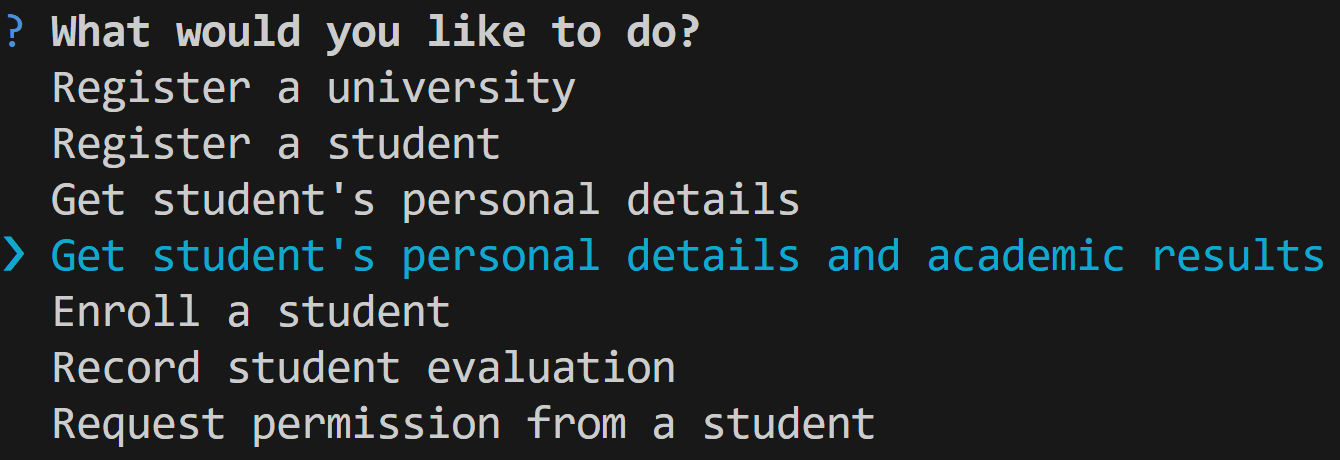
\includegraphics[width=\textwidth]{figures/CLI screen 1.png}
        \caption{Sliding menu}
        \label{sfig:cliDesign1}
    \end{subfigure}
    \hfill
    \begin{subfigure}{.60\textwidth}
        \centering
        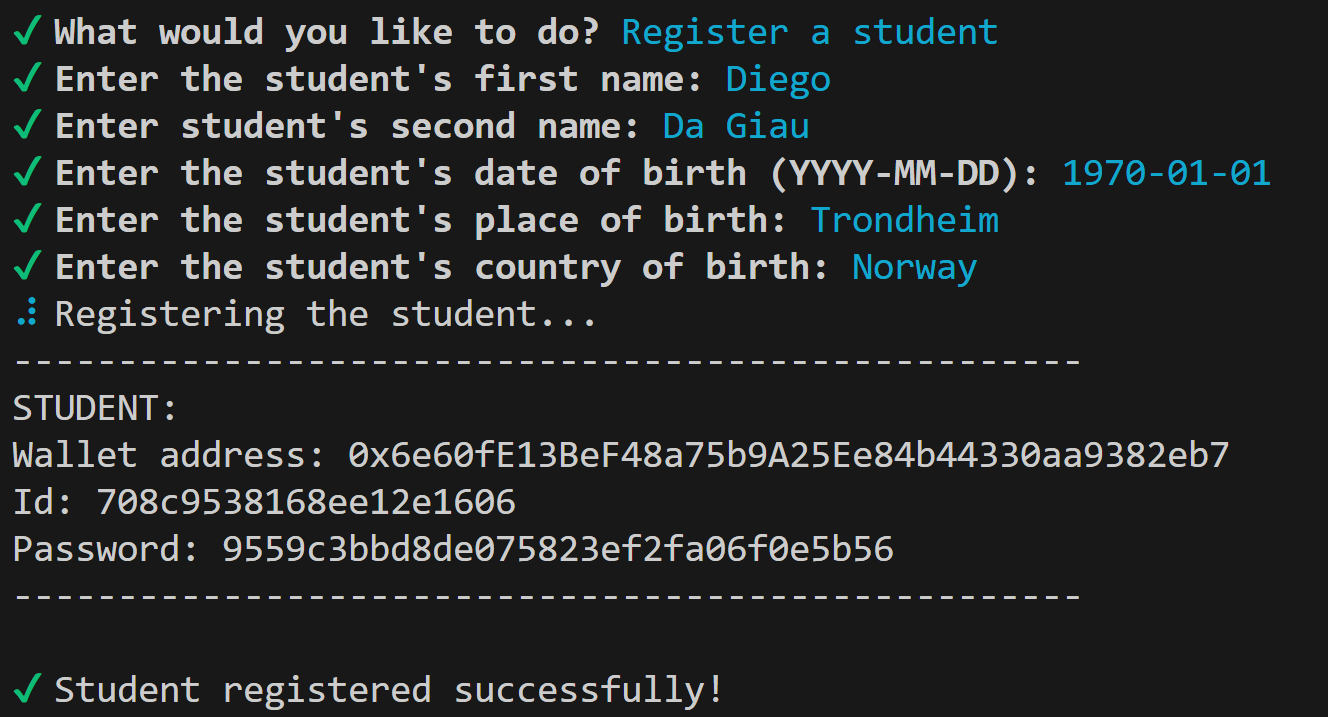
\includegraphics[width=\textwidth]{figures/CLI screen 2.png}
        \caption{User input and visual feedbacks}
        \label{sfig:cliDesign2}
    \end{subfigure}
    \caption[Different aspects of the \acrshort{cli} interface.]{Snapshots of the \acrshort{cli} interface}
    \label{fig:clifigs}
\end{figure}

\subsection{CLI Features}
The \acrshort{cli} exposes all the features outlined in \cref{fig:useCaseCli}. Users can:
\begin{itemize}
    \item Submit a request to register a university in the \acrshort{ew} system.
    \item Register a new student.
    \item Retrieve a student’s personal details.
    \item Retrieve a student’s details and academic results.
    \item Enrol a student in a new course.
    \item Evaluate a student.
    \item Request permissions from a student.
    \item Verify existing permissions.
\end{itemize}
Additionally, the \acrshort{cli} provides options to change the current university and exit the program.

\begin{figure}
  \centering
  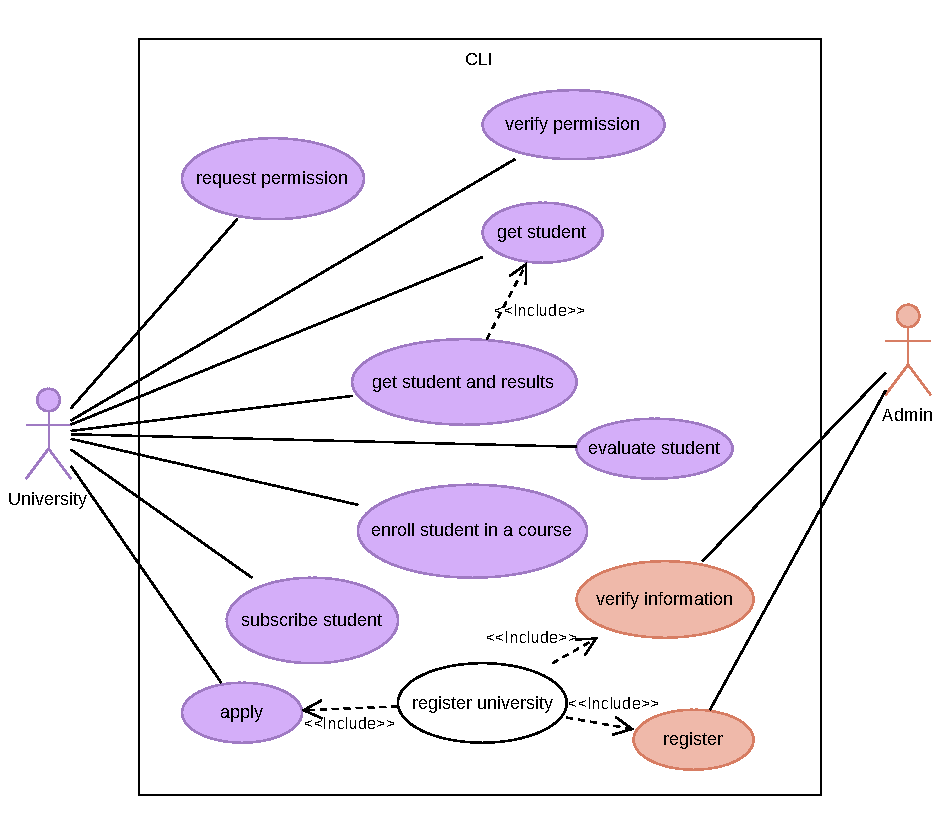
\includegraphics[width=0.8\textwidth]{figures/CLI use case diagram.pdf}
  \caption[\acrshort{cli} use case diagram]{Use case diagram representing the functionalities provided by the \acrshort{cli}.}
  \label{fig:useCaseCli}
\end{figure}

\subsubsection{Testing environment initialization}
Before performing any operation, the \acrshort{cli} must initialize a local blockchain test network by deploying the following smart contracts:
\begin{itemize}
    \item EntryPoint
    \item StudentDeployer
    \item UniversityDeployer
    \item Paymaster
    \item StudentsRegister
\end{itemize}
The \textit{Paymaster} contract then must also be funded to sponsor users' transactions.

In public testnets or in production networks, this initialization step would be unnecessary, as the contracts would already be deployed. Their addresses would be hardcoded in the \acrshort{cli}, \acrshort{sdk} and browser extension.

\subsubsection{University registration}
\label{sssec:applyEw}
To apply to the \acrshort{ew} system, a university must provide its name, country, and short name. Upon receiving these parameters, the \acrshort{cli} generates a random private key, which becomes the private key of the university's \acrshort{eoa}. The \acrshort{eoa} is then set as the active identity used to execute the subsequent operations on behalf of the university. Upon successful completion, the the \acrshort{cli} returns the generated private key, which is essential for accessing the its \acrshort{sca}. In a real \acrshort{lms}, this private key must be securely stored and used to initialize the \acrshort{eoa} wallet when interact with the \acrshort{sdk}. 

To enable immediate interaction with the EntryPoint contract on the local testnet, the \acrshort{cli} also funds the university's \acrshort{eoa}. This step is unnecessary in public or production networks, where the bundler covers transaction fees and is reimbursed by the Paymaster.

\subsubsection{Register a new student}
To register a student, the  university provides their name, surname, date of birth, place of birth and country of birth. The \acrshort{cli} then invokes the \acrshort{sdk} to create the student's smart account and credentials, which are returned to the university (\cref{sfig:cliDesign2}). The \acrshort{sca} address uniquely identifies the student and must be stored by the university, as it is required for all future interactions. 

The \acrshort{cli} also funds the student's \acrshort{eoa} for local testing. The wallet address is obtained from the login credentials, as explained for the browser extension in \cref{sec:browserExtensionDesign}.

\subsubsection{Student Information Retrieval}
To retrieve a student's personal information or full academic record, university must provide the student's smart account address. The \acrshort{cli} then returns the requested data.

\subsubsection{Enrol and evaluate}
To enrol or evaluate a student, the university must provide the smart account address and course code. Enrolment also requires the course name, number of \acrshort{ects} and degree course name. Evaluation requires the evaluation date and, optionally, the path to a certificate file. Since the \acrshort{sdk} allows enrolment in or evaluation of multiple courses at once, the \acrshort{cli} also supports submitting multiple records in a single command.     

\subsubsection{Permissions: Request and Verification}
To access or modify student's academic records, the university must request permission. The \acrshort{cli} requires the student's \acrshort{sca} address and the type of permission (read or write).
The \acrshort{cli} also includes the option to verify whether the university currently has read or write permission for a specific student.

\subsubsection{Changing University and Exiting the \acrshort{cli}}
These functionalities are unique to the \acrshort{cli} and are included for convenience. To change the active university, the user provides the private key of another registered university. To exit the \acrshort{cli}, the user selects the corresponding menu option.

\subsubsection{Administrator Functionalities}
The \acrshort{cli} also includes admin functionalities, as outlined  in \textit{FR 1} of \cref{tab:funcReq}, to facilitate system testing. Specifically, the administrator can:
\begin{itemize}
    \item Review the information submitted in university registration request.
    \item Approve and register universities in the system.
\end{itemize}
These functionalities are embedded within the university registration option. A university is automatically registered when its information is provided by the user during the registration process.

\subsection{Data validation}
All user input is validated using regular expressions and formatting rules. For instance, wallet addresses and private keys are validated based on length and structure\footnote{Private keys must start with \textit{0x} and be followed by 64 hexadecimal characters; addresses by 42.}. Strings are validated to fall within predefined length limits. Dates must follow the \textit{YYYY-MM-DD} format to avoid ambiguity and must be after January 1, 1970, as they are stored as Unix timestamps (unsigned integers). \acrshort{ects} values are checked to ensure they are valid integers or floating-point numbers within acceptable limits. Since the smart contracts store \acrshort{ects} as integers scaled by 100 (see \cref{sec:studentContract} for further details), the \acrshort{cli} ensures the values will not cause overflow during storage.

\chapter*{\bibname}
\printbibliography[heading=none]

\appendix
\chapter{GitHub Repository}
\label{chap:gitHub}

\url{https://github.com/NTNU-IDI/eduwallet-eduwalletdiego}
\chapter{Figma Prototype Link}
\label{chap:figma}

\url{https://www.figma.com/design/aZrmR2thWfRGKQWDQbZE9C/EduWallet?node-id=125-95&t=gQwA5a4uDzRy8jBl-1}
\chapter{Base Paymaster Contract}
\label{chap:basePaymaster}

\lstinputlisting[%
    caption={BasePaymaster smart contract},
    language=Solidity,
    numbers=left,
]{listings/BasePaymaster.sol}

\end{document}
